% !TeX root = ../document.tex
\documentclass[../document.tex]{subfiles}
\lstset{inputpath=sections}
\begin{document}

	\subsection{Principal Component Analysis}
	So far we have focused on supervised learning and go on now to unsupervised learning, where we don't know the response variables. So the goal cannot be prediction rather to have insight into the structure of the data matrix X. We focus on the two most popular approaches.

	\paragraph{PCA}
	We have seen the use of PCA in chapter 6 in the context of principal components regression, where it was used to find subspaces which are, for the given reduced dimension, the closest to the original data. Since PCA only uses the predictor variables and not the response variable Y, it is considered an unsupervised technique, which can be used for data exploration.

	\paragraph{What are principal components?}
	PCA finds a low-dimensional representation of a data set that contains a much as possible of the original variation. The higher the variation, the more interesting that dimension is.\\
	The first principal component of a set of features \(X_{1},X_{2},...,X_{p}\) is the normalized linear combination of the features which results in the largest variance.
	\begin{equation}
	\begin{split}
		X&=\left[\begin{matrix}
			x_{11} & \dots & x_{1p}\\
			\vdots &\ddots& \vdots\\
			x_{n1} & \dots & x_{np}
			\end{matrix}\right]\\
		Z_{1}=X \cdot \phi_1 &= \left[\begin{matrix}
			x_{11} & \dots & x_{1p}\\
			\vdots &\ddots& \vdots\\
			x_{n1} & \dots & x_{np}
			\end{matrix}\right] \cdot \left[\begin{matrix}
				\phi_{11}\\
				\phi_{21}\\
				\vdots\\
				\phi_{p1}
			\end{matrix}\right]
		= \left[\begin{matrix}
			z_{11}\\
			\vdots\\
			z_{n1}
			\end{matrix}\right]\\
		z_{i1}&=\phi_{11}X_{i1}+\phi_{21}X_{i2}+...+\phi_{p1}X_{ip}\\
		\text{1. principal component} = \phi_{1} &= \left[\begin{matrix}
			\phi_{11}\\
			\phi_{21}\\
			\vdots\\
			\phi_{p1}
		\end{matrix}\right], \qquad \phi_{ij}\text{=loadings}\\
		\sum_{j=1}^{p}\phi_{j1}^2&=1 \qquad \text{(unit vector)}\\
		\text{goal: find } &\phi_1 \text{ to maximize }Var(Z_1)\\
	\end{split}
	\end{equation}
	\(\phi_{11}, \phi_{21},...,\phi_{p1}\) are called the \textbf{loadings} of the first principal component. Together these make up the principal component loading vector. $Z$ is effectively $X$, transposed into a new coordinate system where the axes are principal components. In case dimension reduction is employed, some accuracy is lost (dimensionality of $Z_i$ is $<p$).
	The goal is to find the linear combination of the sample feature values, such that the largest sample variance results.
	\begin{equation}
	\begin{split}
		\text{maximize }(\frac{1}{n}\sum_{i=1}^{n}(\sum_{j=1}^{p}\phi_{j1}x_{ij})^2)\text{ subject to }\sum_{j=1}^{p}\phi_{j1}^2=1\\
		z_{i1}=\phi_{11}x_{i1}+\phi_{21}x_{i2}+\dots+\phi_{p1}x_{ip}
	\end{split}
	\end{equation}
	The resulting \(z_{i1},...,z_{n1}\) are called the \textbf{scores} of the first principal component. Geometrically speaking, the loading vector \(\phi_{1}\) defines a direction in the feature space along which the data vary the most. After the first principal component \(Z_{1}\) as been determined, the second principal component \(Z_{2}\) can be calculated. Again, it is a linear combination of \(X_{1},...,X_{p}\) that has maximal variance and a loading vector of length one. This requires \(Z_{2}\) to be uncorrelated with \(Z_{1}\) and that implies that \(\phi_{2}\) needs to be orthogonal to \(\phi_{1}\).

	\paragraph{Scaling the variables}
	Usually the data matrix $X$ is column centered($E[X_i]=0$) and this will bring the centroid to the origin with no side-effects. \textbf{PCA is sensitive to scaling}, which may happen naturally due to differences in units. To combat this, the input data may be scaled down by its variance beforehand:
	\begin{equation}
		X'_i=\frac{X_i}{Var(X_i)}
	\end{equation}

	\paragraph{Unique - up to a sign}
	Since each principal component loading vector identifies an optimal direction in p-dimensional space, it is unique, up to its sign. Similarly, the score vectors $Z$ are unique up to a sign flip, since the variance of $Z$ is the same as the variance of ($-Z$).

	\paragraph{The proportion of variance}
	But the question is now how much information (variance) is lost by projecting the p-dimensional data set onto the first few principal components?
	\begin{equation}
		\sum_{j=1}^{p}Var(X_{j})=\sum_{j=1}^{p}\frac{1}{n}\sum_{i=1}^{n}x_{ij}^2
	\end{equation}
	This is the total variance for a column-centered data matrix X.
	\begin{equation}
		\frac{1}{n}\sum_{i=1}^{n}z_{im}^2=\frac{1}{n}\sum_{i=1}^{n}(\sum_{j=1}^{p}\phi_{jm}x_{ij})^2
	\end{equation}
	This is the variance of the m-th principal component. Hence the proportion of variance explained (PVE) by the m-th principal component can be calculated as shown below:
	\begin{equation}
		PVE=\frac{\sum_{i=1}^{n}(\sum_{j=1}^{p}\phi_{jm}x_{ij})^2}{\sum_{j=1}^{p}\sum_{i=1}^{n}x_{ij}^2}
	\end{equation}
	This term is always between 0 and 1.

	\paragraph{Linear Regression vs PCA}
	\begin{center}
		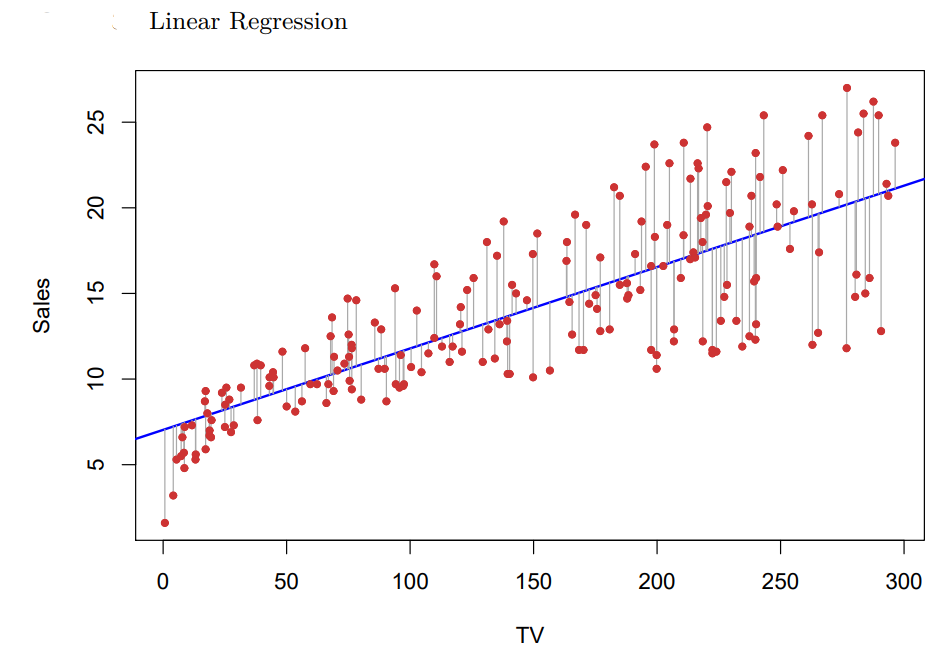
\includegraphics[width=.4\textwidth]{pictures/linear_regression}
		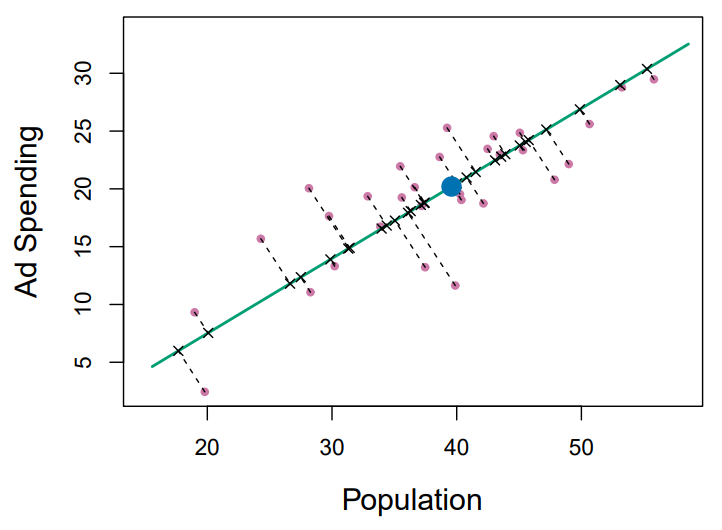
\includegraphics[width=.4\textwidth]{pictures/PCA}\\
		Linear regression's RSS (left) vs PCA (right)
	\end{center}
	PCA and linear regression lead to the same optimal solution, however where LR uses RSS to measure the vertical distance to the ideal line, PCA uses the perpendicular distance and re-defines the data points in terms of this relation (each datapoint $x$ is re-defined in terms of its position along the line $\rightarrow z$)
	\begin{center}
		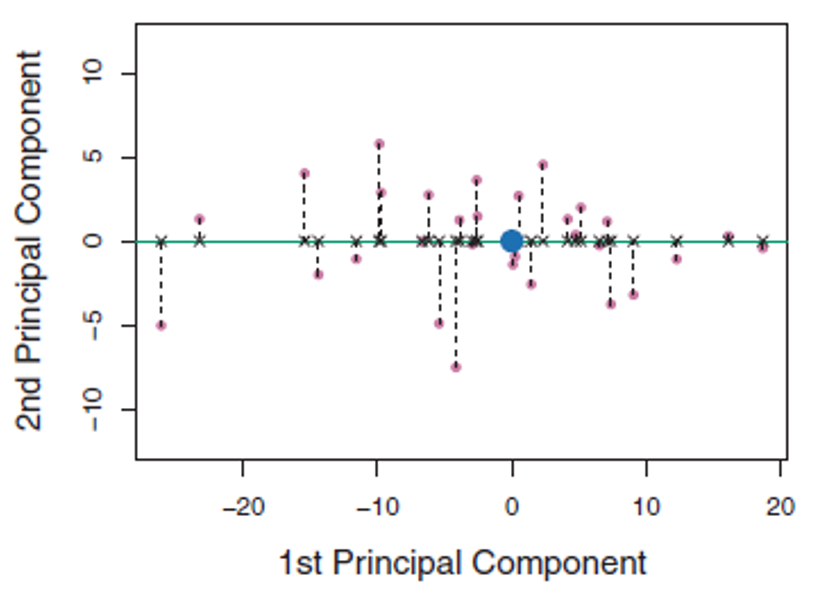
\includegraphics[width=.4\textwidth]{pictures/PCA_2}\\
		PCA after 1. PC is applied.
	\end{center}


	\paragraph{How many principal components should be used?}
	In general a nxp data matrix X has min(n-1,p) distinct principal components. Usually the goal is to reduce the dimensionality significantly, by focusing on the first few principal components.\\
	This is highly subjective but unfortunately the best we can do for unsupervised data exploration. In a supervised setting, a form of cross-validation would be the proper way of selecting the number of components.

	\sectionbreak
	\subsection{Clustering Methods}

	\paragraph{Clustering}
	Technique for finding subgroups or clusters in a data set. The goal is to partition the data set into distinct groups, such that the observation in each group are similar to each other and observations from different groups are quite different from each other. PCA and clustering seek to simplify the data via a small number of summaries. We will focus on the two most popular approaches. Note that one can cluster the n observations (on the basis of the features) or one can cluster the p-features (on the basis of the observations) but we will cluster observations, but simply transposing X will cluster features.

	\paragraph{K-means clustering}
	This is a simple and elegant method for partitioning a data set into K distinct clusters. The basic idea of K-means clustering is, that a good clustering is one for which the within-cluster variation is as small as possible.
	\begin{equation}
	\begin{split}
		\text{minimize}&\left(\sum_{k=1}^{K}W(C_{k})\right)\\
		W(C_{k})&=\frac{1}{|C_{k}|}\sum_{i,i'\in C_{k}}\sum_{j=1}^{p}(x_{ij}-x_{i'j})^2
	\end{split}
	\end{equation}
	There are many ways of defining within-cluster variation, but the most popular is the one above. Unfortunately, solving this problem optimally is extremely time consuming for reasonable n and K.

	\paragraph{K-means clustering algorithm}
	\begin{enumerate}
		\item Randomly assign a number, from 1 to K, to each of the observations. These serve as initial cluster assignment for the observations.
		\item Iterate until the cluster assignments stop changing:
		\begin{itemize}
			\item For each of the K clusters, compute the cluster centroid. The kth cluster centroid is the vector of the p feature means for the observations in the kth cluster.
			\item Assign each observation to the cluster whose centroid is closest (Euclidean distance)
		\end{itemize}
	\end{enumerate}
	Since the final solution depends on the random initialization, it is important to run K-means several times with different random initializations. After each convergence, the quality of the solution is known, since the goal is to minimize the resulting total within-cluster variation.

	\paragraph{Hierarchical clustering}
	K-means requires the specification of the number of clusters K. Hierarchical clustering does not require such a choice and presents a family of possible clustering solutions and associated number of clusters K in a tree structure, a so called dendrogram.
	\begin{figure}
		\centering
		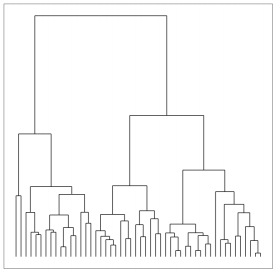
\includegraphics[width=0.7\linewidth]{pictures/dendrogram}
		\caption{Dendrogram}
		\label{fig:dendrogram}
	\end{figure}

	The focus will be on bottom-up or agglomerative clustering. For any two observations, we can look for the point in the tree where branches containing those two observations are first fused. The height of this fusion indicates how different the two observations are. By cutting horizontally across, the dendrogram results in a number of cluster. The higher this cut, the fewer cluster remain, the lower the cut the more cluster result. The underlying assumption is, that the data can be meaningfully clustered in a hierarchical way, if this is not true, this is not the right tool.

	\paragraph{Hierarchical clustering algorithm}
	\begin{enumerate}
		\item Begin with n observations and a measure (Euclidean distance) of all the
		\(
		\begin{pmatrix}
			n\\2
		\end{pmatrix} = n(n-1)/2
		\)
		 pairwise dissimilarities. Treat each observation as its own cluster.
		\item For i = n, n-1,...,2:
		\begin{itemize}
			\item Examine all pairwise inter-cluster dissimilarities among the i clusters and identify the pair of clusters that are least dissimilar (that is, most similar). Fuse these two clusters. The dissimilarity between these two clusters indicates the height in the dendrogram at which the fusion should be placed.
			\item Compute the new pairwise inter-cluster dissimilarities among the i-1 remaining clusters.
		\end{itemize}
	\end{enumerate}
	The notion of dissimilarity needs to be extended to a pair of groups of observation (linkage)
	\begin{itemize}
		\item [Complete] Maximal inter-cluster dissimilarity. Compute all pairwise dissimilarities between the observations in cluster A and the observations in cluster B, and record the largest of these dissimilarities.
		\item [Single] Minimal inter-cluster dissimilarity. Compute all pairwise dissimilarities between the observations in cluster A and the observations in cluster B, and record the smallest of these dissimilarities. Single linkage can result in extended, trailing clusters in which single observations are fused one-at-a-time.
		\item [Average] Mean inter-cluster dissimilarity. Compute all pairwise dissimilarities between the observations in cluster A and the observations in cluster B, and record the average of these dissimilarities.
		\item [Centroid] Dissimilarity between the centroid for cluster A and the centroid for cluster B. Centroid linkage can result in undesirable inversions.
	\end{itemize}
	Average, complete and single are the most popular. Centroid linkage is often used in genomics.

	\paragraph{Practical issues}
	Small decisions with big consequences, validating the obtained clusters and other considerations are issues. Other considerations are for example that outliers have an effect on the result and will highly distort clusters.

\end{document}
